% --------------------------------------------------------------------------------
\pagebreak
\begin{exercise}
Beweisen Sie:
\FloatBarrier
\begin{figure}[h!]
    \centering
    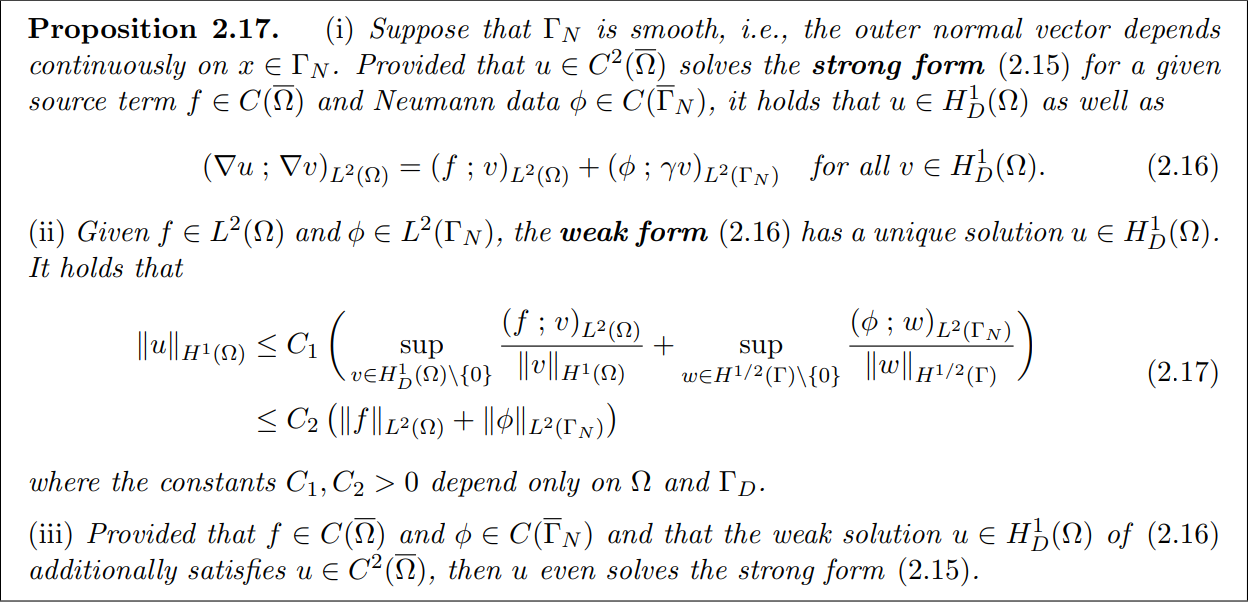
\includegraphics[width = 0.95 \textwidth]{Proposition 2.17.png}
\end{figure}
\FloatBarrier

\end{exercise}

% --------------------------------------------------------------------------------

\begin{solution}

Mixed Boundary Value Problem:



\begin{figure}[h!]
    \centering
    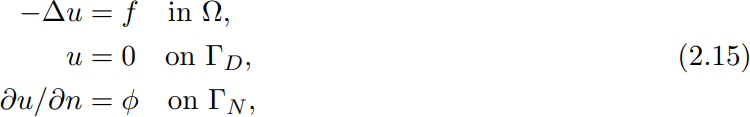
\includegraphics[width = 0.55 \textwidth]{(2.15).png}
\end{figure}

\begin{enumerate}[label = (\roman*)]

    \item $u \in C^2(\overline{\Omega})$ und $u = 0$ auf $\Gamma_D$.

    \begin{align*}
        \implies
        u
        \in
        \Bbraces{v \in C^1(\overline{\Omega}): v|_{\Gamma_D} = 0}
        =:
        C_D^1(\overline{\Omega})
        \subseteq
        \overline
        {
            C_D^1(\overline{\Omega})
        }^{
            \norm[H^1(\Omega)]{\cdot}
        }
        =:
        H^1_D(\Omega)
    \end{align*}

    \includegraphicsboxed
    [mehrdimensionales Analogon der partiellen Integration - Partielle Differentialgleichungen - Jüngel]
    [mAdpI-PD-J]
    {mehrdimensionales Analogon der partiellen Integration.png}

    Wir wissen bereits aus Proposition 1.1. dass die gewünschte
    Gleichheit zumindest für Funktionen aus $C_D^1(\overline{\Omega})$ gilt.
    Für festes $u$ sind die linke und rechte Seite der Gleichung jeweils
    lineare, stetige Funktionale auf $H_D^1(\Omega)$.
    Genauer gilt aufgrund der Stetigkeit des Trace-Operators
    \begin{align*}
      (\nabla u; \nabla v)_{L^2(\Omega)} &\leq \|\nabla u\|_{L^2(\Omega)}\|\nabla v\|_{L^2(\Omega)}
      \leq \|\nabla u\|_{L^2(\Omega)}\|v\|_{H_D^1(\Omega)} \\
      (f;v)_{L^2(\Omega)} + (\phi;\gamma v)_{L^2(\Gamma_N)} &\leq
      \|f\|_{L^2(\Omega)}\|v\|_{L^2(\Omega)} + \|\phi\|_{L^2(\Gamma_N)}\|\gamma v\|_{L^2(\Gamma_N)}
      \leq \|f\|_{L^2(\Omega)}\|v\|_{L^2(\Omega)} + C\|\phi\|_{L^2(\Gamma_N)}\|v\|_{H_D^1(\Omega)} \\
      &\leq (\|f\|_{L^2(\Omega)} + C\|\phi\|_{L^2(\Gamma_N)})\|v\|_{H_D^1(\Omega)}.
    \end{align*}
    Für beliebiges $v \in H_D^1(\Omega)$ wähle nun eine Folge
    $(v_n)_{n \in \N} \subset C_D^1(\overline{\Omega})$ mit $v_n \xrightarrow{n \to \infty} v$.
    Aufgrund der Stetigkeit der obigen Operatoren folgt
    \begin{align*}
    (\nabla u; \nabla v)_{L^2(\Omega)}
    &= \lim_{n \to \infty} (\nabla u; \nabla v_n)_{L^2(\Omega)} \\
    &= \lim_{n \to \infty} (f;v_n)_{L^2(\Omega)} + (\phi;\gamma v_n)_{L^2(\Gamma_N)}
    = (f;v)_{L^2(\Omega)} + (\phi;\gamma v)_{L^2(\Gamma_N)}.
    \end{align*}
    \item

    \begin{figure}[h!]
        \centering
        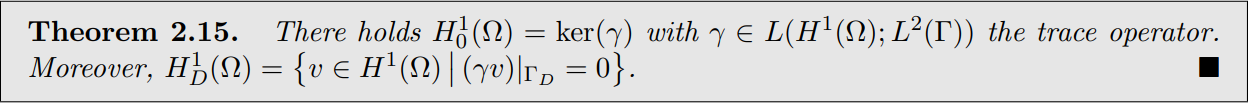
\includegraphics[width = 0.95 \textwidth]{Theorem 2.15.png}
    \end{figure}

    \begin{figure}[h!]
        \centering
        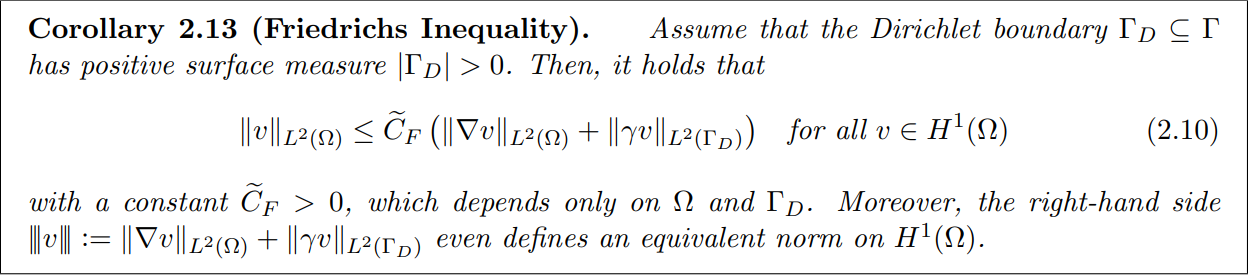
\includegraphics[width = 0.95 \textwidth]{Corollary 2.13 (Friedrichs Inequality).png}
    \end{figure}

    Laut Theorem 2.15 und Corollary 2.13 (Friedrichs Inequality), bildet die linke Seite von (2.16) ein Skalarprodukt (in $u$ und $v$) auf dem abgeschlossenen $H_D^1(\Omega)$.
    Wir erhalten also einen Hilbertraum.
    Die rechte Seite von (2.16) bildet ein lineares Funktional (in $v$).

    \begin{figure}[h!]
        \centering
        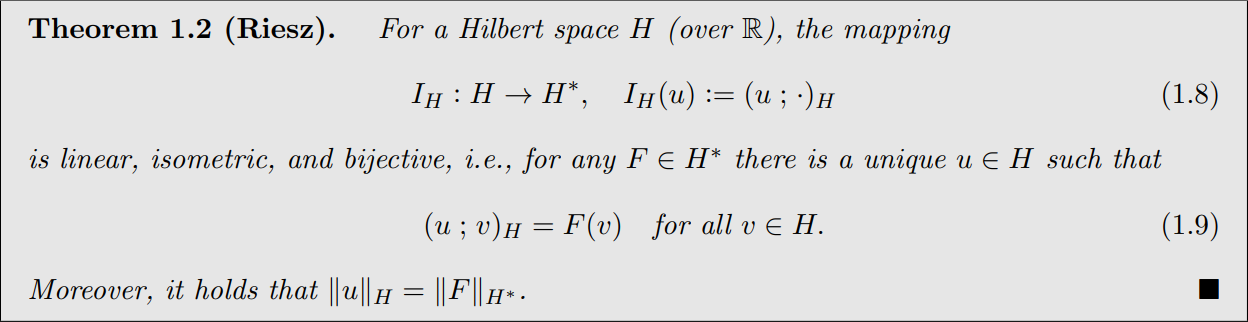
\includegraphics[width = 0.95 \textwidth]{Theorem 1.2 (Riesz).png}
    \end{figure}

    Laut Theorem 1.2 (Riesz), folgt daher die eindeutige Existenz einer Lösung $u \in H_D^1(\Omega)$ von (2.16).
    Wir erinnern uns nun an die Exercise 9 und den darin definierten Raum $H^{1/2}(\Gamma)$ mit seiner Norm $\norm[H^{1/2}(\Gamma)]{\cdot}$.

    \begin{figure}[h!]
        \centering
        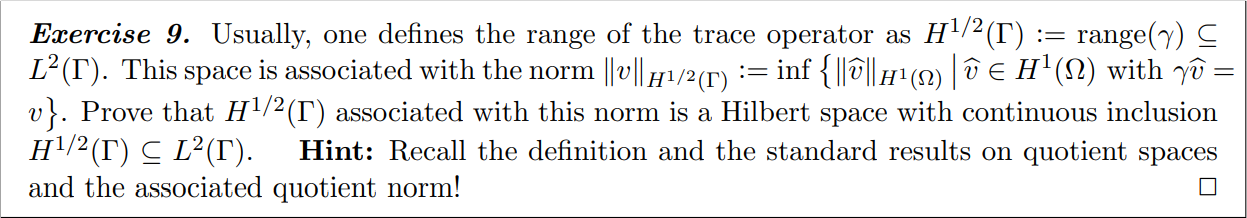
\includegraphics[width = 0.95 \textwidth]{Exercise 9.png}
    \end{figure}

    \begin{multline*}
        \implies
        \norm[L^2(\Omega)]{\nabla u}^2
        =
        (\nabla u; \nabla u)_{L^2(\Omega)}
        \stackrel{\text{(2.16)}}{=}
        (f; u)_{L^2(\Omega)}
        +
        (\phi; \gamma u)_{L^2(\Gamma_N)} \\
        \leq
        \sup_{v \in H_0^1(\Omega) \setminus \Bbraces{0}}
        \frac
        {
            (f; v)_{L^2(\Omega)}
        }{
            \norm[H^1(\Omega)]{v}
        }
        \norm[H^1(\Omega)]{u}
        +
        \sup_{w \in H^{1/2}(\Gamma) \setminus \Bbraces{0}}
        \frac
        {
            (\phi; w)_{L^2(\Gamma_N)}
        }{
            \norm[H^{1/2}(\Gamma)]{w}
        }
        \underbrace
        {
            \norm[H^{1/2}(\Gamma)]{\gamma u}
        }_{
            \leq
            \norm[H^1(\Omega)]{u}
        }
    \end{multline*}

    Mit Corollary 2.13 (Friedrichs Inequality), Cauchy-Schwarz-Bunjakowski, und der Stetigkeit (d.h. Beschränktheit) von $\gamma$ erhalten wir die gewünschten Ungleichungen.

    \begin{align*}
        \norm[H^1(\Omega)]{u}^2
        &= \|u\|_{L^2(\Omega)}^2 + \|\nabla u\|_{L^2(\Omega)}^2
         \stackrel{\text{2.13}}{\leq}
        (1 + \widetilde{C}_F^2)\|\nabla u\|_{L^2(\Omega)}^2 \\
        &\leq
        (1 + \widetilde{C}_F^2)
        \pbraces
        {
            \sup_{v \in H_0^1(\Omega) \setminus \Bbraces{0}}
            \frac
            {
                (f; v)_{L^2(\Omega)}
            }{
                \norm[H^1(\Omega)]{v}
            }
            +
            \sup_{w \in H^{1/2}(\Gamma) \setminus \Bbraces{0}}
            \frac
            {
                (\phi; w)_{L^2(\Gamma_N)}
            }{
                \norm[H^{1/2}(\Gamma)]{w}
            }
        } \norm[H^1(\Omega)]{u} \\
        & \stackrel{\text{CSB}}{\leq}
        \widetilde{C}_F
        \pbraces
        {
            \sup_{v \in H_0^1(\Omega) \setminus \Bbraces{0}}
            \frac
            {
                \norm[L^2(\Omega)]{f}
                \norm[L^2(\Omega)]{v}
            }{
                \norm[H^1(\Omega)]{v}
            }
            +
            \sup_{w \in H^{1/2}(\Gamma) \setminus \Bbraces{0}}
            \frac
            {
                \norm[L^2(\Gamma_N)]{\phi}
                \norm[L^2(\Gamma_N)]{w}
            }{
                \norm[H^{1/2}(\Gamma)]{w}
            }
        } \norm[H^1(\Omega)]{u}\\
        & =
        \widetilde{C}_F
        \Bigg (
            \norm[L^2(\Omega)]{f}
            \underbrace
            {
                \sup_{v \in H_0^1(\Omega) \setminus \Bbraces{0}}
                \frac
                {
                    \norm[L^2(\Omega)]{v}
                }{
                    \norm[H^1(\Omega)]{v}
                }
            }_{
                \leq 1
            }
            +
            \norm[L^2(\Gamma_N)]{\phi}
            \underbrace
            {
                \sup_{w \in H^{1/2}(\Gamma) \setminus \Bbraces{0}}
                \frac
                {
                    \norm[L^2(\Gamma_N)]{w}
                }{
                    \norm[H^{1/2}(\Gamma)]{w}
                }
            }_{
                =
                \norm{\gamma}
                <
                \infty
            }
        \Bigg ) \norm[H^1(\Omega)]{u}\\
        & \leq
        \pbraces
        {
            \widetilde{C}_F
            \max \Bbraces{1, \norm{\gamma}}
        }
        \pbraces
        {
            \norm[L^2(\Omega)]{f}
            +
            \norm[L^2(\Gamma_N)]{\phi}
        }\norm[H^1(\Omega)]{u}
    \end{align*}

    \item Wir berechnen mit Partieller Integration nach Korollar 2.12, da ja $u \in C^2(\overline{\Omega})$, für $v \in H_D^1(\Omega)$:

    \begin{multline*}
      (f;v)_{L^2(\Omega)} + (\phi;\gamma v)_{L^2(\Gamma_N)} = (\nabla u; \nabla v)_{L^2(\Omega)}
      =
      \Int[\Omega]{\nabla u \nabla v}{x}
      =
      -\Int[\Omega]{\Delta u v}{x} + \Int[\partial \Omega]{v(\nabla u \cdot n)}{s} \\
      =
      -(\Delta u; v)_{L^2(\Omega)}
      + \Int[\Gamma_N]{v \frac{\partial u}{\partial n}}{s}
      + \underbrace{\Int[\Gamma_D]{v \frac{\partial u}{\partial n}}{s}}_{0}
      =
      -(\Delta u; v)_{L^2(\Omega)} + \left(\frac{\partial u}{\partial n}; \gamma v\right)_{L^2(\Gamma_N)}
    \end{multline*}

    Da nun $u$ auch $(2.16)$ löst erhalten wir durch bilden der Differenz:

    \begin{align*}
      0 = (f + \Delta u, v)_{L^2(\Omega)} + (\phi - \frac{\partial u}{\partial n}, \gamma v)_{L^2(\Gamma_N)}
    \end{align*}

    Da dies für beliebige $v \in H_D^1(\Omega)$ gilt, schließen wir daraus, dass beide Summanden schon $0$ sind.
    Wegen $\mathrm{D}(\Omega) \subset H^1_0(\Omega) \subset H^1_D(\Omega)$ und da $f + \Delta u \in C(\Omega) \subset L^1_{loc}(\Omega)$ folgt damit aus dem Fundamentallemma der Variationsrechnung

    \begin{align*}
        -\Delta u = f \quad \text {f.ü. in} \quad \Omega
    \end{align*}

    und wegen der Stetigkeit sogar überall.
    Mit der selben Argumentation (da $\Gamma_N$ offen ist) erhalten wir

    \begin{align*}
      \frac{\partial u}{\partial n} = \phi \quad \text{auf} \quad \Gamma_N
    \end{align*}

    Um noch $u = 0$ auf $\Gamma_D$ zu zeigen, bemerken wir, dass $u \in H^1_D(\Omega)$ und wegen der Stetigkeit $\gamma u = u|_{\Gamma}$ also

    \begin{align*}
      0 = (\gamma u)|_{\Gamma_D} = u|_{\Gamma_D}
    \end{align*}
\end{enumerate}

\end{solution}

% --------------------------------------------------------------------------------
